\newpage
\chapter{Flight Test}
\label{chap:flight_test}

\section{Flight Objectives and Planning}
%write for each subsystem

For EPS: Test if suitable power could be supplied to the motors confirming plausibility of providing enough solar power for flight, test of EPS telemetry and telecommand in-flight,  

\section{Flight Results}
%write for each subsystem



\begin{figure}[H]
\centering
\includegraphics[width=0.7\textwidth]{figures/fig_FlightTest1_1}
\caption{First U-SPACE flight test}
\label{fig:FlightTest1_1}
\end{figure}

\begin{figure}[H]
\centering
\includegraphics[width=0.7\textwidth]{figures/fig_FlightTest1_2}
\caption{First U-SPACE flight test}
\label{fig:FlightTest1_2}
\end{figure}


\subsection{Flight results for ITPU}

Shortly before the flight test the BB failed. The attempted provisory fix using a BB-xM turned out to unstable during the flight test (see also \ref{sec:changes_itpu}). While trying to fixate cable connections between the BB-xM and the expansion board cable broke and damaged the expansion board unable to repair on the test side. Therefore the test results presented here are taken from the pre-flight test which was done in the facilities of LTU Kiruna when the original BB was still operational.

\begin{figure}
\centering
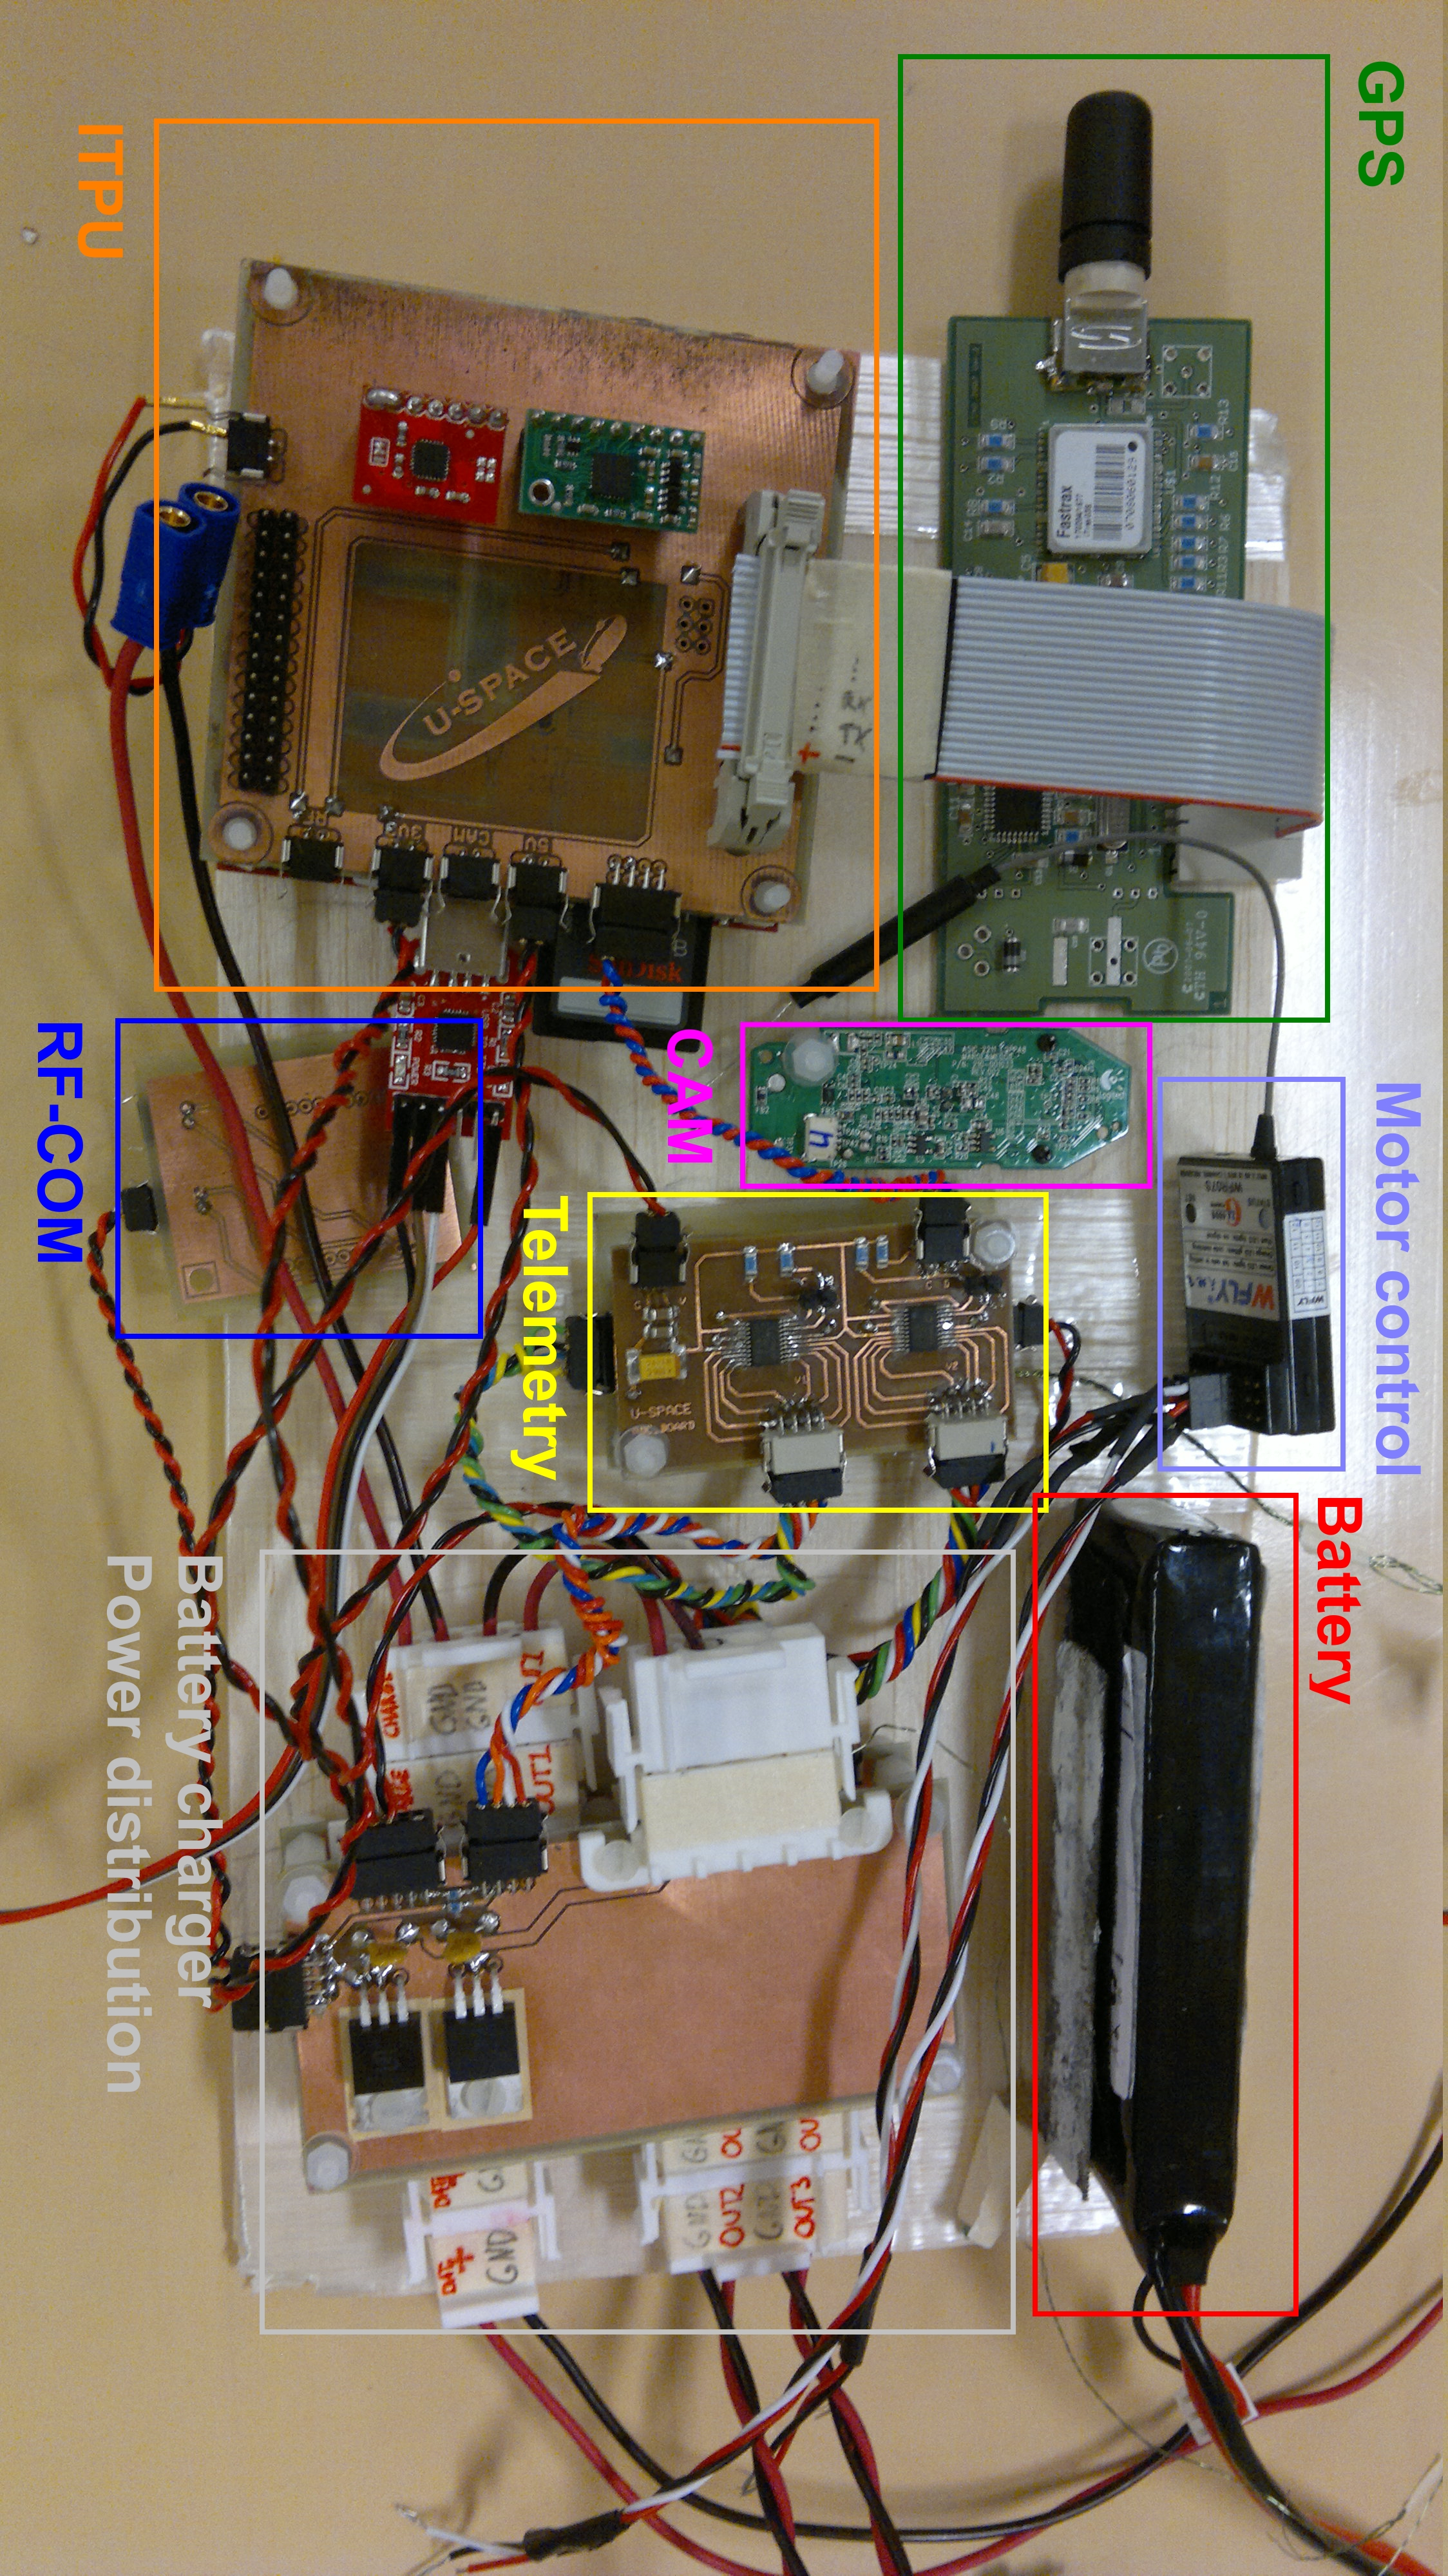
\includegraphics[width=0.55\textheight]{figures/full-system-setup}
\caption{Full system setup}
\label{fig:FlightTest1_1}
\end{figure}

An image of the full system setup including all electronical moduels can be seen in figure . This setup was then mounted into the payload box (see \textcolor{red}{REF!!!}) for testing. As mentioned in section \ref{sec:changes_itpu}, operating both the ADCs of the telemetry subsystem and the sensors of the attitude determination subsystem on the same I2C-bus caused problems which needed manual reset of the I2C-bus in order to get it working again. Peculiar was that both system worked when only one of the two ADCs where connected to the I2C bus together with the attitude sensors, but failed when both ADCs were connected. As the attempts to enable a second I2C-bus on a different expansion header of the BB were unsuccessful, it was decided to test only with one ADC and in turn loose 8 of the 16 telemetry values of the internal voltages. 

With this decision implemented the testing went successful. The wireless connection to the groundstation could be established (for more see \textcolor{red}{REF TO OMAIR}). After calibration of the magnetometer, the attitude determination system was able to determine the attitude stabily and produce the roll-, pitch- and yaw-angles for the telemetry system. When receiving the corresponding signal from the communication module the camera could be activated and shoot either single images or multiple images with a set period (fastest 1~s) and save them to the onboard sd-card.  


\section{Discussions and Future Recommendations}
%write for each subsystem
%
EPS: Due to connector issues, no telemetry was available during flight, thus detailed information of power consumption were not obtained. However, at full thrust, the system has in laboratory shown to draw around 2 x 7.5 A. At a voltage of approximately 7.0 V this corresponds to 105 W power delivered to the motors. According to \cite{website:ModelMotors}, the motors have a relatively poor efficiency of around 67\%. In \cite{CDR} the \ac{EPS} was designed to deliver minimum 40 W of continuous solar power. With these flight results, to allow continuous flight, the size of the solar array should be increased by at least a factor 2.5-3.

The BCR should be re-designed to allow higher output currents. 

A battery with higher voltage should be used - increasing power distribution efficiency and most likely also motor efficiency.
